\documentclass[
   ngerman          % neue deutsche Rechtschreibung
  ,a4paper          % Papiergrösse
  ,12pt             % Schriftgrösse
  ,pdftex
%  ,disable         % Todo-Markierungen auschalten
]{scrreprt}

\usepackage[utf8]{inputenc}        % UTF-8 codierte Dateien

\usepackage[T1]{fontenc}

\usepackage{bericht}

\usepackage{gradientframe}

\usepackage{colortbl}

\usepackage{rotating}

\usepackage{eurosym}

\usepackage{paralist}

\usepackage{enumitem}

\usepackage{rotating}

\usepackage{multirow}

\usepackage{multicol} 

\usepackage{arydshln}

\usepackage{color}

\usepackage{subfigure}

\usepackage{setspace}
\onehalfspacing

\usepackage{listings}             % Include the listings-package for Code
%%\lstset{language=[Sharp]C} % Set your language (you can change the language for each code-block optionally)

\setlength{\parindent}{0em} 

\lstset{
language=csh,
basicstyle=\normalsize\ttfamily,
numbers=left,
numberstyle=\tiny,
numbersep=5pt,
numberstyle=\scriptsize,
tabsize=2,
extendedchars=true,
breaklines=true,
frame=b,
stringstyle=\color{blue}\ttfamily,
showspaces=false,
showtabs=false,
xleftmargin=17pt,
framexleftmargin=17pt,
framexrightmargin=5pt,
framexbottommargin=4pt,
commentstyle=\color{green},
morecomment=[l]{//}, %use comment-line-style!
morecomment=[s]{/*}{*/}, %for multiline comments
showstringspaces=false,
morekeywords={ abstract, event, new, struct,
as, explicit, null, switch,
base, extern, object, this,
bool, false, operator, throw,
break, finally, out, true,
byte, fixed, override, try,
case, float, params, typeof,
catch, for, private, uint,
char, foreach, protected, ulong,
checked, goto, public, unchecked,
class, if, readonly, unsafe,
const, implicit, ref, ushort,
continue, in, return, using,
decimal, int, sbyte, virtual,
default, interface, sealed, volatile,
delegate, internal, short, void,
do, is, sizeof, while,
double, lock, stackalloc,
else, long, static,
enum, namespace, string},
keywordstyle=\color{red},
identifierstyle=\color{black},
backgroundcolor=\color{white},
}

\definecolor{editorGray}{rgb}{0.95, 0.95, 0.95}
\definecolor{editorOcher}{rgb}{1, 0.5, 0} % #FF7F00 -> rgb(239, 169, 0)
\definecolor{editorGreen}{rgb}{0, 0.5, 0} % #007C00 -> rgb(0, 124, 0)

\usepackage{minted}

\usepackage{float}
\restylefloat{figure}

\definecolor{javared}{rgb}{0.6,0,0} % for strings
\definecolor{javagreen}{rgb}{0.25,0.5,0.35} % comments
\definecolor{javapurple}{rgb}{0.5,0,0.35} % keywords
\definecolor{javadocblue}{rgb}{0.25,0.35,0.75} % javadoc

\renewcaptionname{ngerman}{\abstractname}{Kurzzusammenfassung}


%%%%%%%%%%%%%%%%%%%%%%%%%%%%%%%%%%%%%%%%%%%%%%%%%%%%%%%%%%%%%%%%%%%%%%%%%%%%%%%
%% Angaben zur Arbeit
%%%%%%%%%%%%%%%%%%%%%%%%%%%%%%%%%%%%%%%%%%%%%%%%%%%%%%%%%%%%%%%%%%%%%%%%%%%%%%

\newcommand{\Autor}{Avelina Ott}
\newcommand{\MatrikelNummer}{4386414}
\newcommand{\Kursbezeichnung}{TINF15B4}

\newcommand{\FirmenName}{WebCommerce GmbH}
\newcommand{\FirmenStadt}{Offenburg}
\newcommand{\FirmenLogoDeckblatt}{
\includegraphics[width=3cm]{bilder/DHBW.png}}
\newcommand{\BetreuerFirma}{Markus Schill}
\newcommand{\BetreuerDHBW}{Dr. Werner Geiger}

\newcommand{\Was}{Bachelorarbeit}
\newcommand{\Jahr}{2018}
% Wird auf dem Deckblatt in der Erklärung benutzt

%%%%%%%%%%%%%%%%%%%%%%%%%%%%%%%%%%%%%%%%%%%%%%%%%%%%%%%%%%%%%%%%%%%%%%%%%%%%%%%%%%%%%

% Benutzt man das "biblatex"-Paket, dann muß das hier stehen:
% siehe auch die mit BIBLATEX markierten Zeilen in bericht.sty
\bibliography{literatur}

\begin{document}
\pagenumbering{Roman}
%%%%%%%%%%%%%%%%%%%%%%%%%%%%%%%%%%%%%%%%%%%%%%%%%%%%%%%%%%%%%%%%%%%%%%%%%%%%%%%

\newcommand{\Titel}{Web-to-Print: Export von Terminen in eine kundenspezifische DOCX-Datei}
\newcommand{\AbgabeDatum}{27. August 2018}

\newcommand{\Dauer}{12 Wochen}

\newcommand{\Abschluss}{Bachelor of Science}

\newcommand{\Studiengang}{Angewandte Informatik}

\hypersetup{%%
  pdfauthor={\Autor},
  pdftitle={\Titel},
  pdfsubject={\Was}
}

\begin{titlepage}
\begin{center}
\vspace*{-2cm}
%\FirmenLogoDeckblatt
\hfill
\includegraphics[width=4cm]{bilder/DHBW}\\[2cm]
{\Huge \Titel}\\[2cm]
{\Huge\scshape \Was}\\[2cm]
{\large für die Prüfung zum}\\[0.5cm]
{\Large \Abschluss}\\[0.5cm]
{\large des Studienganges \Studiengang}\\[0.5cm]
{\large an der}\\[0.5cm]
{\large Dualen Hochschule Baden-Württemberg Karlsruhe}\\[0.5cm]
{\large von}\\[0.5cm]
{\large\bfseries \Autor}\\[1cm]
{\large \AbgabeDatum}
\vfill
\end{center}
\begin{tabular}{l@{\hspace{2cm}}l}
Bearbeitungszeitraum	         & \Dauer 			\\
%Matrikelnummer	                 & \MatrikelNummer	\\
Kurs			         & \Kursbezeichnung		\\
Ausbildungsfirma	         & \FirmenName			\\
			         %& \FirmenStadt			\\
Betreuer der Ausbildungsfirma	 & \BetreuerFirma		\\
Gutachter/in der Studienakademie	 & \BetreuerDHBW		\\
\end{tabular}
\end{titlepage}

%%%%%%%%%%%%%%%%%%%%%%%%%%%%%%%%%%%%%%%%%%%%%%%%%%%%%%%%%%%%%%%%%%%%%%%%%%%%%%
% Nur für Bachelorarbeiten einfügen:
\selectlanguage{ngerman}
%\begin{abstract}
\onehalfspacing
\addchap{Abstract}
-------------- Hier kommt das deutsche Abstrakt. ---------------------


-------------- Now following: the abstract  ---------------------
%\end{abstract}

\newpage
\addchap{Sperrvermerk}

\singlespacing
%\small
\noindent Die vorgelegte Bachelorarbeit basiert auf internen, vertraulichen Daten und Informationen des Unternehmens Web Commerce GmbH und ist somit \textbf{urheberrechtlich geschützt}. In diese Arbeit dürfen Dritte, mit Ausnahme der Gutachter und befugten Mitgliedern des Prüfungsausschusses, ohne ausdrückliche Zustimmung des Unternehmens und des Verfassers keine Einsicht nehmen. Eine Vervielfältigung und Veröffentlichung der Bachelorarbeit ohne ausdrückliche Genehmigung – auch auszugsweise – ist nicht erlaubt. \\[3ex]
\copyright\ 2018 \ \Autor
\addchap{Eidesstattliche Erklärung}
Gemäß § 5(3) der „Studien- und Prüfungsordnung DHBW Technik“ vom 29. 9. 2015 versichere ich hiermit, dass ich meine Bachelorarbeit mit dem Thema:
   \begin{quote}
     „\textit{\Titel}“
    \end{quote}
selbstständig verfasst und keine anderen als die angegebenen Quellen und Hilfsmittel benutzt habe. Ich versichere zudem, dass die eingereichte elektronische Fassung mit der gedruckten Fassung übereinstimmt.


\vspace{3cm}
\noindent
\underline{\hspace{10cm}}\\\\
Karlsruhe, 27.08.2018\hspace{4cm}\\\\\\

\tableofcontents           % Inhaltsverzeichnis hier ausgeben
\listoffigures             % Liste der Abbildungen
\listoftables              % Liste der Tabellen
\lstlistoflistings         % Liste der Listings


\lstdefinelanguage{Velocity}
{
  %basicstyle=\ttfamily,
  morestring=[s]{"}{"},
  morekeywords={set, foreach, end, if, else},
  otherkeywords={\#, ., get},
  %moredelim=[s][\color{black}]{>}{<},
  moredelim=[s][\color{red}]{\$}{\ },
  %morecomment=[s][\color{red}]{.}{.},
  %moredelim=[s][\color{red}]{\$}{)},
  %moredelim=[s][\color{red}]{\$}{.},
  morecomment=[s][\color{green}]{.}{(},
  commentstyle=\color{green},
  stringstyle=\color{blue},
  keywordstyle=\color{green}
}

\lstdefinelanguage{HTML5}{
        language=html,
        sensitive=true, 
        alsoletter={<>=-},
        otherkeywords={
        % HTML tags
        <html>, <head>, <title>, </title>, <meta, />, </head>, <body>,
        <canvas, \/canvas>, <script>, </script>, <td>, </td>, <tr>, </tr>, </body>, </html>, <!, html>, <style>, </style>, ><
        },  
        ndkeywords={
        % General
        =,
        % HTML attributes
        charset=, id=, width=, height=,
        % CSS properties
        border:, transform:, -moz-transform:, transition-duration:, transition-property:, transition-timing-function:
        },  
        morecomment=[s]{<!--}{-->},
        tag=[s]
}

\lstset{
numbers = left,
frame = single,
framexleftmargin=15pt,
breaklines=true
}

% Jetzt kommt der "eigentliche" Text
\include{abk}              % Abkürzungsverzeichnis

\pagenumbering{arabic}
%%%%%%%%%%%%%%%%%%%%%%%%%%%%%%%%%%%%%%%%%%%%%%%%%%%%%%%%%%%%%%%%%%%%%%%%%%%%%%
%%%% Befehle in der Arbeit
%%%%%%%%%%%%%%%%%%%%%%%%%%%%%%%%%%%%%%%%%%%%%%%%%%%%%%%%%%%%%%%%%%%%%%%%%%%%%%
\newcommand{\edith}{EDITH}
\newcommand{\cms}{Content-Management-System }
\newcommand{\cmsEdith}{CMS EDITH}
\newcommand{\fluid}{Fluid }
\newcommand{\webco}{Web Commerce GmbH }
\newcommand{\sesam}{Sesam}
\newcommand{\abschnitt}{\newline\newline}

\newcommand{\exkurs}[2]{
\begin{leftbar}
	\textbf{Exkurs - } \textit{#1}: #2 
\end{leftbar}
}

\newcommand{\definition}[2]{
\begin{leftbar}
	\textbf{Definition - } \textit{#1}: #2 
\end{leftbar}
}



%%%% steht für „bla"
\newcommand{\qmUO}[1]{\glqq{}#1\grqq{}}
%%%% steht für "bla"
\newcommand{\qmO}[1]{\glqq{}#1\grqq{}}
\chapter{Einleitung}\label{einleitung}
%\onehalfspacing
\section{Vorstellung der \webco}
Die \webco besteht seit dem Jahr 1999 in Form eines eigenständiges Unternehmens als Full-Service-Internet-Dienstleister. Die Haupttätigkeit der etwa 20 Mitarbeiter besteht in der kontinuierlichen Neu- und Weiterentwicklung von maßgeschneiderten Internet-Anwendungen nach den persönlichen Kundenwünschen. Die Entwicklung des eigenen \cms (kurz CMS) \edith \, begann mit der Firmengründung und wird fortlaufend weiterentwickelt. Auf der Basis von dem \cmsEdith\, läuft das Projekt \qmUO{\sesam}. 
\abschnitt
Das auf \edith-basierte Projekt \qmUO{\sesam} ist ein Baukasten für die Erstellung eigener Webseiten in den Seelsorgeeinheiten der Erzdiözese Freiburg. Neben den Seelsorgeeinheiten nutzen auch Dekanate, Diözese-Anstellen und sonstige Einrichtungen das System.
\abschnitt
Neben dem eigenen \cmsEdith\, wird je nach Projektumfang und -anforderungen das Open-Source \cms TYPO3 eingesetzt.


\section{Problemstellung} \label{problemstellung}
Mit dem Projekt \qmUO{Sesam} unterstützt das Erzbischöfliche Ordinariat Freiburg seine Einrichtung bei der Realisierung eines Internet-Auftrittes. Zum Einsatz kommt das von \webco entwickelte \cmsEdith, welches von derzeit ca. 500 SESAM-Mandanten genutzt wird.
\abschnitt
Ein großer Teil dieser Mandanten verwaltet mit \edith\, die Gottesdienst-Termine und gibt diese auf dem eigenen Internetauftritt aus. Bei vielen werden die verwalteten Termindaten in den individuell gestalteten Pfarrbriefen oder Gemeindebriefen verwendet.

\exkurs{Pfarrbrief}{Als Pfarrbrief oder Gemeindebrief wird ein Heft verstanden, das eine christliche Gemeinde als Informationsmedium periodisch an die Mitglieder der Kirche her ausgibt. Oft bildet ein Grußwort eines Pfarrers oder ein geistlicher Impuls den Beginn. Nachfolgend werden Bericht oder Ankündigungen aus der Gemeindearbeit aufgeführt. Abschließend folgt ein Veranstaltungskalender.}

Bislang steht für die Generierung des individuellen Pfarrbriefes eine sehr einfach gehaltene Export-Funktion zur Verfügung, die jedoch nur wenig Gestaltungsmöglichkeiten bietet. Demgegenüber stehen zahlreiche Pfarrbriefvarianten, die sich hinsichtlich Struktur und Formatierung teilweise erheblich unterschieden.
\abschnitt
Um diese Vielfältigkeit der Pfarrbriefe zu verdeutlichen befinden sich in Abbildung \ref{img:Gemeindebrief} zwei unterschiedliche aussehende Pfarrbriefe, die so in Wirklichkeit existieren.\abschnitt
\begin{figure}[h]
    \caption{Pfarrbriefe}
    \label{img:Gemeindebrief}
        \subfigure[Gottesdienste Juli – August 2017 – Katholische Kirche an der Schutter \cite{KatholischeKirchengemeindeanderSchutter.2017}]{
            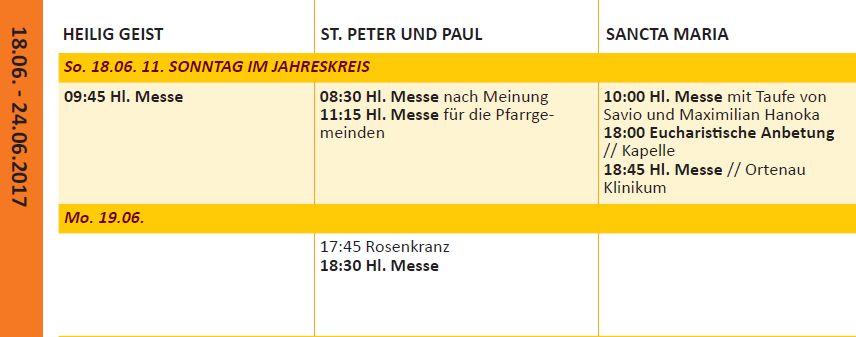
\includegraphics[width=8 cm]{bilder/Gemeindebrief_Schutter.png}
            \label{img:PfarrbriefSchutter} }
        \subfigure[Gemeindebrief vom Mai 2018 – Baden-Baden \cite{Kath.KirchengemeindeBadenBaden.2017}]{
        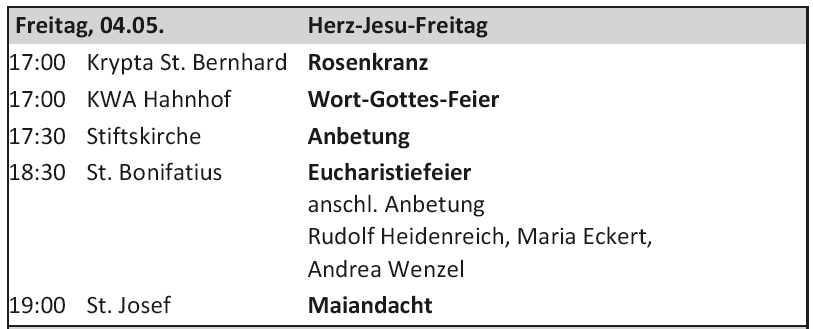
\includegraphics[width=8 cm]{bilder/Gemeindebrief_BadenBaden.png}
        \label{img:PfarrbriefBadenBaden} }
\end{figure}\newline
Sofort ist zu erkennen, dass sich die Pfarrbriefe nicht nur in den Farbe unterscheiden, sondern auch in der Form. Im Pfarrbrief von der Katholischen Kirche an der Schutter, Abbildung \ref{img:PfarrbriefSchutter}, werden die verschiedenen Gottesdienste zuerst auf die verschiedenen Kirchen aufgeteilt und dann den entsprechenden Tagen zugeteilt. Im Gemeindebrief von Baden-Baden, Abbildung\ref{img:PfarrbriefBadenBaden}, hingegen werden die Gottesdienste den Tagen zugeteilt und dann die jeweiligen Kirche einer einzelnen Veranstaltung.
\abschnitt
Um diesen individuellen Ansprüchen der Pfarrblatt-Gestaltung gerecht zu werden, muss das Export-Ergebnis daher manuell aufwändig nach bearbeitet werden. Dafür werden in der Regel die Programme Microsoft Word, Microsoft Publisher oder Adobe InDesign eingesetzt.
\abschnitt
Die mühselige Nacharbeitung erfolgte durch einen nicht technisch begabten Angestellten oder ehrenamtlichen Nutzer der Institutionen mithilfe von \qmUO{Copy \& Paste} in die bevorzugte Software in das gewünschte Design. Die Abbildung \ref{img:AblaufErstellungPfarrbrief} zeigt nochmal den Ablauf für die Erstellung eines Pfarrbriefes. Für diese Arbeit ist der Ablauf im \cmsEdith \, und in der bevorzugten Software, Microsoft Word, Microsoft Publisher oder Adobe InDesign essentiell. An diesen Abschnitten der Erstellung soll eine Verbesserung erfolgen.\abschnitt
\begin{figure}[h]
	\centering
	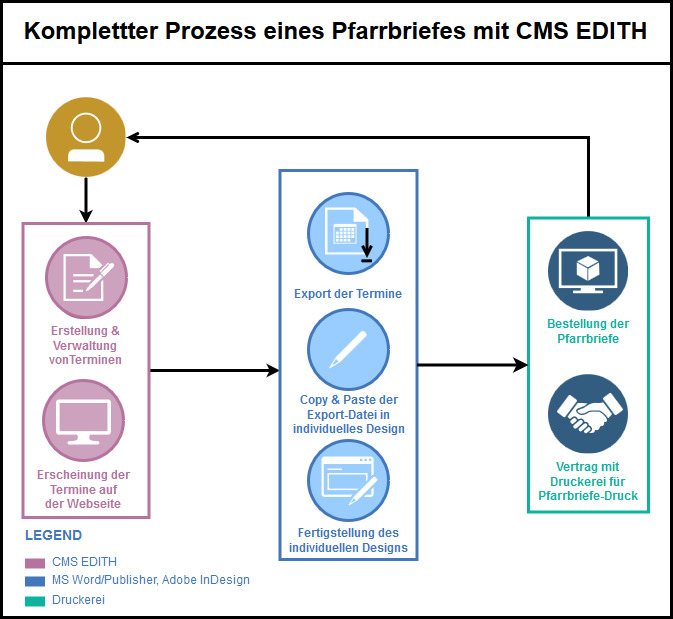
\includegraphics[width=13cm]{bilder/kompletterJetzigerProzess.png}
    \caption{Auflauf zur Erstellung eines Pfarrbriefes mit der bisherigen Export-Funktion}
    \label{img:AblaufErstellungPfarrbrief}
\end{figure} \abschnitt


\section{Motivation} \label{motivation}
Die Motivation ist den Nachbearbeitungsaufwand nach der derzeitigen Export-Funktion für die Mitarbeiter und Mitarbeiterinnen zu verringern. Durch das nachdem Export händische \qmUO{Copy \& Paste} entstehen oft Fehler, die von einer weiteren Person behoben werden müssen oder gänzlich übersehen werden. Zudem ist dieses Verfahren sehr zeitaufwendig und durch mangelhaftes technisches Wissen über die verwendete Software wird die Nacharbeitung nicht erleichtert. \abschnitt
Aufgrund diesem Nachbearbeitungsaufwand kam von vielen Kunden und Mandanten der Wunsch nach einer erweiterten Export-Funktion. Mit der erweiterten Export-Funktion soll ein Dateiformat erzeugt werden, welches alle gewünschten individuellen Design-Entscheidungen und -Vorgaben erfüllt. Das Dateiformat sollte dann in die Softwares Microsoft Word, Microsoft Publisher und Adobe InDesign importiert werden können. Im Rahmen der Projektarbeit 3 wurde diesbezüglich eine Machbarkeitsanalyse durchgeführt, mit dem Ergebnis des Dateiformates \qmUO{DOCX}


\section{Zielsetzung} \label{zielsetzung}
Im Rahmen der Bachelorarbeit soll eine neue Export-Funktion konzipiert werden und in Form eines Prototyps umgesetzt werden. Der Export soll dabei eine möglichst individuelle Ausgabe der Termindaten ermöglichen, sodass deutlich weniger Nachbearbeitungsaufwand für die Mitarbeiter und Mitarbeiterinnen der kirchlichen Einrichtungen anfällt. Im Rahmen der Projektarbeit 3 wurden bereits die Anforderungen an einen solchen Export ermittelt und eine Machbarkeitsanalyse durchgeführt. Es stellt sich dabei heraus, dass das Dateiformat \qmUO{DOCX} in diesem Anwendungskontext sehr gut eignet. \abschnitt
Nach der Fertigstellung des Prototypen soll anhand von den erstellten Anforderungen und Metriken der Prototyp evaluiert werden. So kann festgestellt werden, ob der Prototyp in die Umgebung des \cmsEdith \, integriert werden kann.


\section{Vorgehensweise} \label{vorgehensweise}

\chapter{Anforderungsanalyse} \label{anforderungsanalyse}

--> Welche Spezifikation gilt für das Produkt und wie wurde die Spezifikation ermittelt?

--> Beschreibung des Produktes anhand der wichtigsten Funktionen und Leistungen? --> Eventuell auch Gebrauchsnutzen?

\section{Funktionale Anforderungen} \label{anf:Funktional}



\section{Nicht funktionale Anforderungen} \label{anf:NichtFunktional}






\chapter{Prototyp} \label{prototyp}
Das Ziel dieser Arbeit ist eine erweiterte Export-Funktion anhand eines Prototyp zu konzipieren und umzusetzen. In diesem Kapitel handelt es sich um das Thema der Prototyp. Dabei wird definiert, was ein Prototyp ist, welche Eigenschaft ein Prototyp besitzen soll und welche Arten es existieren. Zusätzlich wird ein standardisierter Ablauf eines Prototyps geschildert. Am Ende werden Vor- und Nachteile eines solchen Vorgehensmodell erläutert und Alternativen vorgestellt.

\section{Definition} \label{prot:Defintion}
\definition{prototype - 1913}{An original or model after which anything is copied; the pattern of anything to be engraved, or otherwise copied, cast, or the like; a primary form; exemplar;archetype}

\definition{prototype - 2004}{1. An original type, form, or instance serving as a basis or standard for later stages. 2. An original, full-scale, and usually working model of a new product or new version of an existing product. 3. An early, typical example}

\section{Eigenschaften} \label{prot:Eigenschaften}



\section{Prototyp-Arten} \label{prot:Prototyparten}


\section{Vorgehen} \label{prot:Prototyp_vorgehen}


\section{Vor- und Nachteile} \label{prot:Prototyp_vorteile}
\chapter{Web-to-Print} \label{web2print}

\section{Definition von Web-to-Print} \label{w2p:Definition}

\section{Web-to-Print vs. Web-to-Publish} \label{w2p:Vergleich}

\section{Bedeutung im Projekt} \label{w2p:Projekt}
\chapter{Template-Engine}

\section{Definition}

\section{Mögliche Template-Engine}

\subsection{Fluid}

\subsection{Smarty}

\subsection{etc.}

\section{Verwendung in diesem Projekt}


\chapter{State of the Art} \label{stateOfTheArt}

--> welche wissenschaftlichen Kenntnisse gibt es bereits, bei der Produktentwicklung berücksichtigt werden sollten?
    --> mögliche Lösungen schon bereits enthalten -> wie wird es bereits woanders umgesetzt?

--> Welche Methode wird angewandt?
    --> hier muss so was rein wie verschiedene Arten von Webt-To-Print, worin sie sich entscheiden, welche Definition verwendet wird etc.

--> hier eventuell ein Vergleich mit bereits existierenden Lösungen von anderen CMS


\section{TYPO3} \label{stand:Typo3}
--> hier kommen Features, Vor- und Nachteile und Probleme rein

\section{Wordpress} \label{stand:Wordpress}
--> hier kommen Features, Vor- und Nachteile und Probleme rein

\section{\edith} \label{stand:Edith}
--> hier kommen Features, Vor- und Nachteile und Probleme rein
\chapter{Planung und Konzept} \label{planung}
--> Welcher Entwicklungsprozess wird gewählt und welche Werkzeuge werden verwendet?


\section{Projektplanung} \label{projektplan}



\section{Konzept} \label{konzept}

\chapter{Umsetzung und Implementierung}\label{implementierung} 


--> Verwendung von Fluid - Warum?
--> Bibliothek für Export - was für welche gibt es?
    --> phpdocx
    --> phpword
    --> warum phpdocx und nicht phpword? --> Verweis auf Projektarbeit 3
    
\chapter{Evaluierung} \label{evaluierung}

\section{Metriken} \label{metriken}
--> wie wird das Produkt erprobt? 
--> Welches Ergebnis zeigt sich?
--> Anhand welcher Metriken wird evaluiert?

\section{Ergebnis} \label{ergebnis}
--> Welche Konsequenzen ergeben sich aus der Erprobung und Evaluierung des Produktes?
\chapter{Zusammenfassung} \label{zusammenfassung}

\section{Fazit} \label{fazit}

\section{Ausblick}\label{Ausblick}


%\include{anhang}
\pagenumbering{Roman}

\addcontentsline{toc}{chapter}{Literaturverzeichnis}
\printbibliography



% Ab hier beginnt der Anhang
\appendix
%\addcontentsline{toc}{chapter}{Anhang}
%\appendix
%\appendixtoc
%\newpage

\renewcommand*{\thesection}{\Alph{section}}
\chapter*{\appendixname}
%\include{anhang}
%\begin{enumerate}[label=\bfseries \LARGE \Alph*, ref=\Alph*]
%	\item Bilder \label{app:bilder}
%   \item Umfrage \label{app:umfrage}
%  \item manueller Testplan \label{app:maTestplan}
%\end{enumerate}

%\bibliographystyle{alphadin}
%\bibliography{literatur}

%%%%%%%%%%%%%%%%%%%%%%%%%%%%%%%%%%%%%%%
% BIBLATEX
% Benutzt man das "biblatex"-Paket, muß man folgendes schreiben:
%\def\refname{Literaturverzeichnis}


%%%%%%%%%%%%%%%%%%%%%%%%%%%%%%%%%%%%%%%

\end{document}